\section{Grundlagen und Methoden} % (fold)
\label{sec:grundlagen_und_methoden}

	In den folgenden Kapiteln wird eine grundlegende Einführung und Definition der Verfahren gegeben, die für den weiteren Verlauf dieser Arbeit von Belang sind.
	Viele dieser Themen können hier nur angerissen werden, da ihre komplette Behandlung den Rahmen und das Ziel des Themas verfehlen würde.
	Für eine genauere Einführung in die einzelnen Themengebiete, wird dem Leser geraten sich mit den genannten Quellen auseinander zu setzen.

	\subsection{Szenenrepresentation} % (fold)
	\label{sec:szenenrepresentation}

		Um realistische Bilder zu generieren, benötigen wir als Eingabe gewisse Daten der physikalischen Objekte, die durch den Beobachter oder auch die Kamera betrachtet werden.
		Für die später betrachteten Algorithmen ist dabei vor allem das Verhalten von Licht auf den Oberflächen dieser Objekte wichtig.
		Der Einfachheit halber wollen wir davon ausgehen, dass das Licht nur in den oberen Schichten eines Körpers mit dessen Material wechselwirkt.
		Für uns ist es also ausreichend, nur die Oberflächen der gegebenen Objekte und nicht deren Inneres zu beschreiben.

		Die Oberflächen realer physikalischer Objekte sind im Allgemeinen beliebig geformt und können nicht in geschlossener Form durch eine Gleichung beschrieben werden.
		Dennoch lassen sie sich im analytischen Sinne durch einfachere Hyperflächen im Raum approximieren.
		Für die Bildgenerierung wählt man für solch eine Fläche meist ein Dreieck.
		Es ist einfach zu beschreiben und flexibel genug um die meisten Objekte beliebig genau zu approximieren.
		Dabei wollen wir entartete Dreiecke, die nur aus einem Punkt oder einer Strecke bestehen, ausschließen, da sie für die betrachteten Render-Verfahren nicht darstellbar sind.
		\begin{definition}[Dreieck]
			Ein Dreieck $\triangle$ wird durch eine Sequenz $(A_\triangle,B_\triangle,C_\triangle)$ von Punkten in $\SR^3$, für die die Menge $\set{B_\triangle-A_\triangle, C_\triangle-A_\triangle}$ linear unabhängig ist, charakterisiert.
			Die Menge $S(\triangle)$ der Punkte des Dreiecks ist definiert durch
			\[
				S(\triangle) \define \im{\varphi_\triangle}
			\]
			Dabei stellt $(M,\varphi_\triangle)$ mit den folgenden Definitionen die Standardparametrisierung der Menge $S(\triangle)$ dar.
			\[
				M \define \set[u+v\leq 1]{(u,v)\in[0,1]^2}
			\]
			\[
				\func{\varphi_\triangle}{M}{S(\triangle)},\qquad \varphi_\triangle(u,v) \define (1-u-v)A_\triangle + uB_\triangle + vC_\triangle
			\]
			Die baryzentrischen Koordinaten $(u,v,w)$ eines Punktes $x\in S(\triangle)$ sind durch die folgenden Eigenschaften gegeben.
			\[
				(u,v)\in M,\qquad w = 1-u-v,\qquad \varphi_\triangle(u,v) = x
			\]
			Die analytische äußere Normale $\mu_\triangle$ ist gegeben durch den Ausdruck
			\[
				\mu_\triangle \define \frac{\crossp{(B_\triangle-A_\triangle)}{(C_\triangle-A_\triangle)}}{\norm{\crossp{(B_\triangle-A_\triangle)}{(C_\triangle-A_\triangle)}}}
			\]
		\end{definition}

		Jedes Dreieck besitzt auf seiner gesamten Fläche eine eindeutige konstante äußere analytische Normale.
		Für die Simulation von globalen Beleuchtungseffekten ist diese Eigenschaft jedoch ein Nachteil, weil die Beleuchtung eines Objektes stark vom Verlauf seiner Normalen abhängt.
		Nähern wir ein Objekt nun durch $n\in\SN$ Dreiecke an, so nähern wir zur Zeit auch den Normalenverlauf des Objektes durch die stückweise konstanten äußeren Normalen der Dreiecke an.
		Der Fehler dieser Approximation tritt in Form eines facettenhaften Musters auf, welcher für das menschliche Auge gut erkennbar ist.
		In Abbildung \ref{fig:facette} wird dieser Effekt genauer an einem Beispiel demonstriert.
		Das Problem kann im Allgemeinen durch eine Interpolation, die die Stetigkeit der Normalen erhält, gelöst werden.
		\begin{definition}[Normalen-Funktion]
			Seien $\triangle$ ein Dreieck und $\func{\nu}{S(\triangle)}{\SR^3}$.
			Dann wird $\nu$ eine äußere Normalen-Funktion auf $\triangle$ genannt, wenn für alle $x\in S(\triangle)$ die folgenden Eigenschaften gelten.
			\[
				\norm{\nu(x)} = 1,\qquad \dotp{\mu_\triangle}{\nu(x)} > 0
			\]
		\end{definition}

		\begin{figure}
			\begin{subfigure}[b]{0.5\textwidth}
				\center
				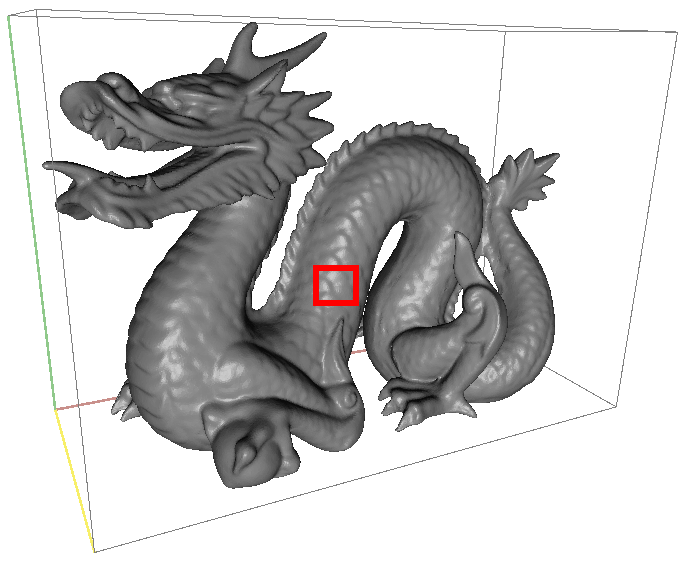
\includegraphics[scale=0.2]{pic/normal_facette-mark.png}
				\caption{}
			\end{subfigure}
			\begin{subfigure}[b]{0.5\textwidth}
				\center
				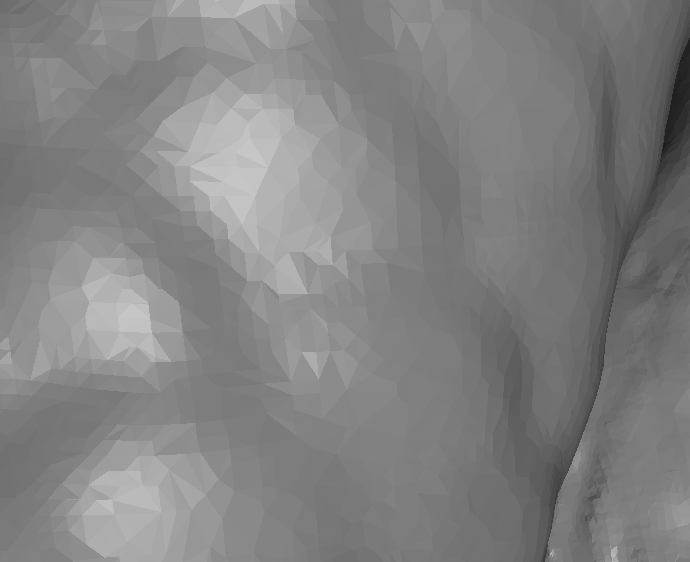
\includegraphics[scale=0.2]{pic/normal_facette-zoom.png}
				\caption{}
			\end{subfigure}
			\caption{Die Bilder zeigen die gerenderte \enquote{Dragon}-Szene. Das rechte Bild entspricht dem roten Bereich des Linken. In dieser Szene werden die Normalen des Objektmodells durch die analytischen Normalen der Dreiecke angenähert. Da das Modell sehr fein trianguliert ist, fällt dies im ersten Bild nicht auf. Zoomt man jedoch mit der Kamera heran werden die Fehler durch die Approximation deutlich und die einzelnen Dreiecke sind mit dem menschlichen Auge auszumachen.}
			\label{fig:facette}
		\end{figure}

		\begin{theorem}[Vertex-Normalen-Funktion]
			Sei $\triangle$ ein Dreieck und seien Normalen $\mu_A, \mu_B, \mu_C \in \SR^3$ an den Punkten des Dreiecks mit den folgenden Eigenschaften für alle $X\in\set{A,B,C}$ gegeben.
			\[
				\norm{\mu_X} = 1,\qquad \dotp{\mu_X}{\mu_\triangle} > 0
			\]
			Dann definiert die Abbildung $\func{\nu}{S(\triangle)}{\SR^3}$ eine stetige Normalen-Funktion auf $\triangle$, wenn für alle $x\in S(\triangle)$ mit den baryzentrischen Koordinaten $(u,v,w)$ die folgende Aussage gilt.
			\[
				\nu(x) = \nu\circ\varphi_\triangle(u,v) \define \frac{w\mu_A + u\mu_B + v\mu_C}{\norm{w\mu_A + u\mu_B + v\mu_C}}
			\]
			Wir nennen $\nu$ in diesem Falle eine Vertex-Normalen-Funktion.
		\end{theorem}

		Durch das Setzen der Normalen an den Eckpunkten eines Dreiecks können wir sicher gehen, dass der Verlauf der Normalen stetig von einem Dreieck zu einem anderen übergeht.
		Ein beipielhafter Verlauf einer Vertex-Normalen-Funktion wird in Abbildung \ref{fig:normal-function} gezeigt.
		Für die in dieser Arbeit betrachteten Effekte und Verfahren reicht diese Art der Normalen-Interpolation aus.
		Dennoch gibt es hier weitere Möglichkeiten, wie zum Beispiel \enquote{Normal Maps}, die eine noch genauere Approximation zu Lasten des Speicherverbrauchs ermöglichen.

		\begin{figure}
			\begin{subfigure}[b]{0.5\textwidth}
				\center
				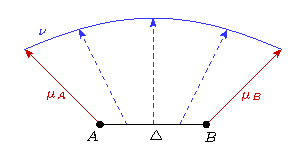
\includegraphics{gg_fig/scheme_normal-function_1.pdf}
				% \caption{Verlauf}
			\end{subfigure}
			\begin{subfigure}[b]{0.5\textwidth}
				\center
				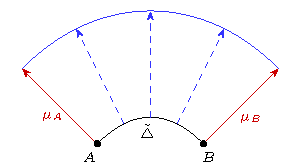
\includegraphics{gg_fig/scheme_normal-function_2.pdf}
				% \caption{approximierte Fläche}
			\end{subfigure}
			\caption{Die erste Skizze auf der linken Seite zeigt den Verlauf einer Vertex-Normalen-Funktion $\nu$ anhand eines Beispiels. $A_\triangle$ und $B_\triangle$ sind dabei die Eckpunkte eines Dreiecks $\triangle$. $\mu_A$ und $\mu_B$ sind die jeweilig gegebenen Vertex-Normalen an den Eckpunkten. Im rechten Bereich der Abbildung ist die durch $\nu$ approximierte gekrümmte Fläche $\tilde{S}(\triangle)$, auf der die Normalen $\nu(x)$ senkrecht stehen, eingezeichnet.}
			\label{fig:normal-function}
		\end{figure}

		Die kleinste Hyperfläche, die wir durch geschlossene Gleichungen beschreiben können und aus derer wir alle weiteren Objekte zusammensetzen, nennen wir \enquote{Primitiv} (engl.: \textit{primitive}).
		Es soll in unserem Falle nicht nur die Informationen des Dreiecks beinhalten, sondern auch Aussagen über dessen Material oder Oberflächenstruktur treffen können.
		Insbesondere muss das Primitiv oder dessen Material also die Reflexion, Absorbtion, Transmission und Emission des Lichts an der Oberfläche beschreiben.
		Für physikalische Materialien gibt es aber je nach den betrachteten Effekten verschiedene verallgemeinerte Varianten der mathematischen Beschreibung.
		Um keine dieser Varianten auszuschließen, soll hier das Primitiv in einer abstrakteren Form definiert werden.
		\begin{definition}[Primitiv]
			Sei $\s{M}$ die Menge der Elemente, die Materialien von Objekten charakterisieren.
			Dann ist ein Primitiv $p$ gerade ein Tupel $(\triangle_p, \nu_p, m_p)$, bestehend aus einem Dreieck $\triangle_p$, einer Normalen-Funktion $\nu_p$ auf $\triangle_p$ und einem Material $m_p\in \s{M}$.
		\end{definition}


		Für die eigentliche Approximation der Oberfläche eines Objektes benötigt man jetzt eine Menge von Primitiven.
		Solch eine Menge wollen wir auch eine \enquote{Szene} (engl.: \textit{scene}) nennen.
		Häufig benötigt man jedoch neben den Lichtquellen, die durch die Materialien der Primitive gegeben sind, noch weitere anders geartete Lichtquellen, die unabhängig von den eigentlichen Primitven der Szene bestehen.
		In unserem Falle wollen wir uns speziell auf die Umgebungsbeleuchtungs-Funktion (engl.: \textit{HDR environment map}) beziehen.
		\begin{definition}[Umgebungsbeleuchtungs-Funktion]
			Sei $n\in\SN$.
			Dann ist eine Umgebungsbeleuchtungs-Funktion definiert als eine auf $\Omega$ integrierbare Abbildung $\func{f}{\Omega}{[0,\infty)^n}$.
		\end{definition}

		Diese Funktion beschreibt das Licht durch $n\in\SN$ ausgewählte Koeffizienten, welches von einer Kugeloberfläche mit quasi unendlich großem Radius in die Szene ausgesandt wird.
		Für einen Punkt der Szene, ist dessen Beleuchtung durch diese Funktion also unabhängig von dessen Position.
		Diese Tatsache wird in Abbildung \ref{fig:hdr_environment_map} wieder an einem Beispiel gezeigt.
		Die eigentliche Definition soll nun durch eine solche Umgebungsbeleuchtungs-Funktion erweitert werden.

		\begin{figure}
			\center
			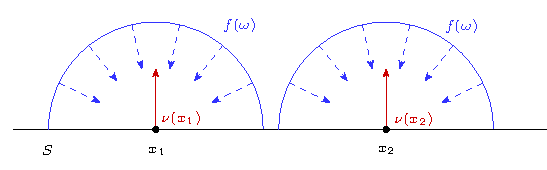
\includegraphics{gg_fig/hdr_environment_map_1.pdf}
			\caption{Die Darstellung zeigt, dass die Beleuchtung zweier Punkte $x_1$ und $x_2$ einer Oberfläche $S$ mit den Normalen $\nu(x_1)$ und $\nu(x_2)$ durch eine Umgebungsbeleuchtungs-Funktion $f$ nur abhängig von der Verdeckung der Punkte und nicht von deren Position ist. Bei $x_1$ und $x_2$ sind also in diesem Falle die gleichen Lichtintensitäten zu messen.}
			\label{fig:hdr_environment_map}
		\end{figure}

		\begin{definition}[Szene]
			Eine Szene $\s{S}$ bezeichnet ein Tupel $(P_\s{S},E_\s{S})$ mit einer endlichen Menge $P_\s{S}$ von Primitiven und einer Umgebungsbeleuchtungs-Funktion $E_\s{S}$.
			Die Menge $S(\s{S})$ der Punkte in der Szene $\s{S}$ sei definiert durch
			\[
				S(\s{S}) \define \bigcup_{p\in P_\s{S}} S(\triangle_p)
			\]
		\end{definition}

	% subsection szenenrepresentation (end)

	\subsection{Raytracing} % (fold)
	\label{sub:raytracing}

		Im einfachsten Falle bezeichnet das Wort \enquote{Raytracing} (engl.: \textit{ray tracing}) einen Algorithmus zur Ermittlung der Sichtbarkeit von dreidimensionalen Objekten bezüglich eines Ursprungpunktes (engl.: \textit{origin}) im Raum.
		Häufig versteht man darunter jedoch auch eine Render-Technik für die Generierung eines gesamten Bildes aus einer gegebenen Szene, die auf dem eben genannten Raytracing-Algorithmus basiert.

		Grundsätzlich gibt es viele Verfahren, um ein Szene auf ein Bild zu rendern.
		Die Erfahrung zeigt aber, dass vor allem in Bereichen, in denen die globalen Beleuchtungseffekte realistisch simuliert werden sollen, Raytracing eine wichtige Grundlage darstellt.
		Der Grund dafür besteht in der Tatsache, dass Raytracing das Sichtbarkeitsproblem löst und durch die Verwendung von Strahlen eine Basis für die Lichtberechnung im Sinne der geometrischen Optik bereitstellt.
		\begin{definition}[Sichtbarkeitsproblem]
			Sei $\s{S}$ eine Szene.
			Dann ist die Sichtbarkeitsfunktion von $\s{S}$ die folgende Abbildung.
			\[
				\func{V_\s{S}}{\SR^3\times S(\s{S})}{\set{0,1}}
			\]
			\[
				V_\s{S}(o,x)=
				\begin{cases}
					1 &: S(\s{S}) \cap \set[\gamma\in(0,1)]{(1-\gamma)o + \gamma x} = \emptyset \\
					0 &: \m{sonst}
				\end{cases}
			\]
			Das Sichtbarkeitsproblem beschreibt dann die Aufgabe diese Funktion für gegebene Szenen und Parameter zu evaluieren.
		\end{definition}

		\begin{figure}[h]
			\center
			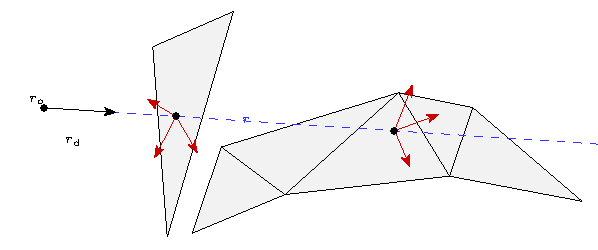
\includegraphics{gg_fig/ray_tracing_1.pdf}
			\caption{Die Abbildung zeigt eine Skizze, welche das Sichtbarkeitsproblem und den Raytracing-Algorithmus verdeutlicht. Die grau melierten Dreiecke sollen die gegebene Szene $\s{S}$ darstellen. Der ausgesendete Strahl $r=(r_\m{o},r_\m{d})$ trifft in der Szene genau zwei Punkte $x_1$ und $x_2$. Dabei wird $x_2$ durch $x_1$ verdeckt. Es gilt also $V_\s{S}(r_\m{o},x_1)=1$ und $V_\s{S}(r_\m{o},x_2)=0$.}
			\label{fig:ray_tracing-1}
		\end{figure}

		Die Sichtbarkeitsfunktion gibt an, ob der Oberflächenpunkt $x$ vom Beobachtungspunkt $o$ aus in gerader Linie gesehen werden kann oder ob zwischen diesen Punkten ein Primitiv den Punkt $x$ verdeckt.
		Daran anknüpfend besteht die Basis des Raytracing-Verfahrens auf dem Aussenden von \enquote{Strahlen} (engl.: \textit{ray}) bezüglich eines Ursprungspunktes.
		Für diese Strahlen kann der Schnittpunkt mit der Szene ermittelt werden.
		Liegt der Schnittpunkt zwischen $o$ und $x$, so beträgt der Wert der Sichtbarkeitsfunktion $0$ ansonsten $1$.
		Die Sichtbarkeitsfunktion kann somit für alle gegebenen Parameter durch Raytracing berechnet werden.
		Abbildung \ref{fig:ray_tracing-1} zeigt diese Methode anhand einer Skizze.
		\begin{definition}[Strahl]
			Ein Strahl $r$ sei gerade durch ein Tupel $(r_\m{o},r_\m{d})$ mit einem Ursprungspunkt $r_\m{o}\in\SR^3$ und einer Richtung $r_\m{d}\in\SR^3\setminus\set{0}$ charakterisiert. Die Menge $S(r)$ der Punkte des Strahls ist gegeben durch das Bild der Parametrisierung $([0,\infty),\varphi_r)$
			\[
				S(r) \define \im{\varphi_r},\qquad \func{\varphi_r}{[0,\infty)}{\SR^3},\qquad \varphi_r(t)\define r_\m{o} + tr_\m{d}
			\]
			Die Menge aller Strahlen sei mit $R$ bezeichnet.
		\end{definition}

		Die vollständige Evaluierung von $V_\s{S}$ ist jedoch häufig nicht nötig.
		In Abbildung \ref{fig:ray_tracing-1} ist klar, dass alle Punkte von $r$, die hinter $x_1$ liegen von dem Beobachtungspunkt $r_\m{o}$ aus nicht sichtbar sind.
		Beim eigentlichen Raytracing-Algorithmus macht man sich dies zu Nutze und berechnet für eine vorgegebene Richtung nur den nächsten Schnittpunkt.
		Alle weiteren Schnittpunkte können ignoriert werden, da sie vom Strahl aus nicht erreicht werden.
		\begin{definition}[Raytracing-Funktion]
			Sei $\s{S}$ eine Szene.
			Dann ist die Raytracing-Funktion der Szene $\s{S}$ gegeben durch die folgende Abbildung.
			\[
				\func{\m{rt}_\s{S}}{R}{(0,\infty]}
			\]
			\[
				\m{rt}_\s{S}(r) \define
				\begin{cases}
					\min\set[r(t)\in S(\s{S})]{t\in(0,\infty)} &: S(\s{S})\cap \varphi_r((0,\infty)) \neq \emptyset \\
					\infty &: \m{sonst}
				\end{cases}
			\]
		\end{definition}

		Wie bereits erwähnt, erweitert man diesen Algorithmus häufig mit der Berechnung eines gesamten Bildes, indem man für jeden Pixel des Bildes einen oder mehrere Strahlen durch einen analogen virtuellen Pixel im Szenenraum schießt und die Raytracing-Funktion für diese evaluiert.
		Abbildung \ref{fig:ray_tracing-2} zeigt dieses Verfahren anhand einer Skizze.
		Um gleichzeitig das Shading zu ermöglichen, ermittelt man nicht nur den Schnittpunkt, sondern auch in welchem Primitiv sich dieser befindet und welche baryzentrischen Koordinaten er besitzt.
		Die Implementierung des Raytracing-Verfahrens soll hier nicht gezeigt werden, da eine einfache naive Implementierung meistens einen zu großen Rechenaufwand darstellt und die hier verwendete optimierte Variante weit über das Thema dieser Arbeit hinausgeht.

		\begin{figure}
			\center
			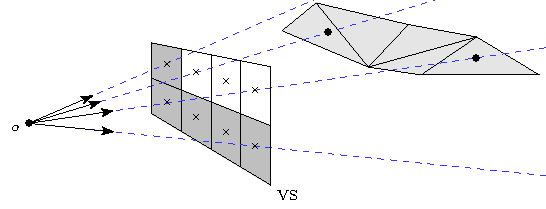
\includegraphics{gg_fig/ray_tracing_2.pdf}
			\caption{In der Skizze ist ein typisches Render-Verfahren auf der Basis des Raytracing-Algorithmus dargestellt. Bezüglich eines Beobachtungspunktes $o$ wird durch jeden Pixel eines virtuellen Bildschirms $\m{VS}$ ein Strahl geschossen und dessen Raytracing-Funktion evaluiert. Gibt es keinen Schnittpunkt, so wird der Pixel meistens schwarz gefärbt. Ansonsten kann zum Beispiel die Farbe des getroffenen Objektes angezeigt werden. Der Übersicht wegen sind im Bild nur vier der eigentlich acht Strahlen sichtbar.}
			\label{fig:ray_tracing-2}
		\end{figure}

	% subsection raytracing (end)

	\subsection{Photometrie} % (fold)
	\label{sub:photometrie}

		Ein physikalischer Körper $K$ mit der Oberfläche $\partial K$ und äußerer Normalen-Funktion $\mu$ sendet aufgrund verschiedener physikalischer Effekte, wie zum Beispiel Reflexion, elektromagnetische Wellen aus.
		Für die Simulation von Beleuchtungseffekten ist es nun nötig die Abhängigkeit der Abstrahlung für verschiedene Wellenlängen $\lambda\in(0,\infty)$, verschiedene Punkte $x\in\partial K$ und verschiedene Richtungen $\omega\in\Omega$ zu betrachten.
		Dafür führen wir die sogenannte \enquote{spektrale Strahldichte} (engl.: \textit{spectral radiance}) ein.
		Sie gibt an, wie viel Energie pro Zeit, pro Wellenlängenänderung, pro Flächenelement und pro Raumwinkel abgestrahlt wird.
		Sind also messbare Teilmengen $\Lambda\subset (0,\infty)$, $U\subset \partial K$ und $S\subset\Omega$ gegeben, so kann man die spektrale Strahldichte über die abgegebene Strahlungsleistung der Oberfläche $U$ in den Raumwinkelbereich $S$ definieren.
		Die zugehörige Abbildung ist dann wie folgt gegeben.
		\[
			\func{\s{L}}{(0,\infty)\times\partial K\times \Omega}{[0,\infty)}
		\]
		\[
			\Phi(\Lambda,U,S) \definedby \integral{\Lambda}{}{ \integral{U}{}{ \integral{S}{}{ \s{L}(\lambda,x,\omega)\abs{\dotp{\mu(x)}{\omega}} }{\omega} }{\sigma(x)} }{\lambda}
		\]
		Abbildung \ref{fig:radiance} zeigt noch einmal eine Skizze, welche die Struktur dieser Abbildung verdeutlicht.
		Der Erfahrung nach stellt die spektrale Strahldichte für das menschliche Auge die sinnvollste messbare Größe für die empfundene Helligkeit einer Oberfläche bezüglich eines Beobachtungspunktes dar.

		\begin{figure}[h]
			\center
			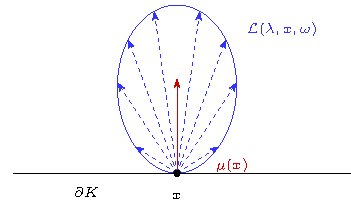
\includegraphics{gg_fig/radiance_1.pdf}
			\caption{Die Skizze stellt ein qualitatives Beispiel einer spektralen Strahldichte $\s{L}$ dar, die an einem Punkt $x$ auf der Oberfläche $\partial K$ und für eine Wellenlänge $\lambda$ eine Verteilung in Abhängigkeit von $\omega$ auf der Einheitskugel besitzt. In der Abbildung ist dabei die Abstrahlung nur erlaubt, wenn $\dotp{\omega}{\mu}>0$, wobei $\mu$ die äußere Normale im Punkt $x$ beschreibt.}
			\label{fig:radiance}
		\end{figure}

		Eine weitere Größe, die wir hier einführen möchten, ist die sogenannte \enquote{Bestrahlungsstärke} (engl.: \textit{irradiance}).
		Sie wird vor allem bei der noch folgenden Konstruktion der Irradiance Maps benötigt werden.
		\[
			\func{\s{E}}{(0,\infty)\times\partial K}{[0,\infty)},\qquad \s{E}(\lambda,x) \define \integral{\Omega}{}{ \s{L}(\lambda,x,\omega)\abs{\dotp{\mu(x)}{\omega}} }{\sigma(\omega)}
		\]
		Die Bestrahlungsstärke quantifiziert die Energie pro Zeit, pro Wellenlänge und pro Flächenelement an einem Punkt auf der Oberfläche des Objektes.

		Für die weiteren Algorithmen und Implementierungen reicht es eine entkoppelte Abbildung zu betrachten, welche für jeden Punkt einer Szene und jede gegebene Richtung die Strahldichte bestimmt.
		Später wird dies die Funktion sein, die wir durch Radiance Maps annähern wollen.
		\begin{definition}[Strahldichte-Funktion]
			Sei $\s{S}$ eine Szene.
			Dann ist die Abbildung $\func{L_\s{S}}{S(\s{S})\times \Omega}{[0,\infty)}$ eine Strahldichte-Funktion von $\s{S}$.
		\end{definition}

	% subsection photometrie (end)

% section grundlagen_und_methoden (end)